\documentclass{article}
\usepackage[utf8]{inputenc}
\usepackage[a4paper, total={15cm, 24cm}]{geometry}
\usepackage{amsmath}
\usepackage{amssymb}
\usepackage{fancyhdr}
\usepackage{lastpage}
\usepackage{graphicx}
\usepackage[english]{babel}
\usepackage{float}
\usepackage{url}
\usepackage{kpfonts}
\usepackage{amsmath}
\usepackage{cancel} % For cancellation lines (for fractions)
\usepackage{lmodern}
\usepackage{xcolor}
\usepackage{mathtools}
\usepackage{amsthm}
\usepackage{fdsymbol}
\usepackage{listings}
\usepackage{appendix}

\usepackage{parskip} % til at venstre align alt
\graphicspath{ {./images/} }  


\title{
    Fagprojekt 01666 \\
    \large{Symbolic evaluation of sums using neural networks}
}
\author{Mikael H. Hoffmann (s214753) \and Hugo M. Nielsen (s214734) \and Christian V. Kjær (s211469) \and Jacob Tuxen (s194572) \and Jonas D. Larsen (s205829)}
\date{}

\begin{document}

\maketitle
\newpage

\section{Abstract}
\newpage

\tableofcontents
\newpage

\section{Introduction}



\subsection{Background}
% Section til hvad der startede ideen
% Indhold:
%       Facebooks paper's indhold
Deep Learning for symbolic Mathematics\footnote{FODNOTE TIL ATIKKEL} is a paper written by Facebooks AI Research department and is the foundation to our project. The article focuses on the use of a neural network to solve complicated symbolic integration, with very successful results even out performing leading mathematical software as maple and Wolfram Mathematica on some of there own test data. Figure \ref{facebooks_res1} shows some of the results from Facebook. Facebook managed to get 98.4 percentage correct results on its own test data witch is significantly better than the best mathematical software programs. The neural network that facebooks used, outputs 50 results and then ranks them according to how correct it thinks each result is. Meaning Beam 1 is the result that the neural network has found, to be the best solution. Beam size x then means that the correct answer to an symbolic integral was within the first x best solutions found by the network.  

\begin{figure}[H]    
% kan være der skal findes et bedre kval pic
    \centering
    \label{facebooks_res1}
    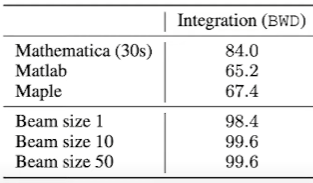
\includegraphics{facebooksBWDvsMathematica.png}
    \caption{insert cap}
\end{figure}



BWD Means the dataset used to train the neural network, was created by taking the derivative of an equation as input to the neural network. Since it takes less computational power for a mathematical software to compute the derivative of a given equation than the integral. 

It need to be noted that the test dataset of 5000 integration equations, was generated by the same software as the set the neural network was trained on. Meaning that it is unsure if the network will perform as good on integration equations produced outside of the original software. 

Whats really interesting about the paper is that it manage to solve equations that could not be solved by the model it was trained on. This is whats lay grounds for our project, we want to use similar methods as Facebook AI Research on a neural network to train it on symbolic evaluation of sums.  

\subsection{Neural Network}\label{neural_network}
% ved ikke om den her skal før Background
% Section til hvad et neuralt netværk
% Indhold:
%       Opbyggningen af et neuralt netværk
%       Input Output (seq2seq)
%       vægtene
\subsubsection{Embedding layers - not sure about the placement of this in the introduction!}
% Feel free to change anything! 
Traditionally when working with Natural Language Processing (NLP) each word from a dictionary with a given length $n = 7$ can be written using a vector

\begin{equation}
    \begin{split}
        \text{car} &=
        \begin{bmatrix}
            1 & 0 & 0 & 0 & 0 & 0 & 0
        \end{bmatrix}, \\
        \text{driving} &= 
        \begin{bmatrix}
            0 & 0 & 0 & 1 & 0 & 0 & 0
        \end{bmatrix}.
    \end{split}
\end{equation}

And here we can identify two problems:

\begin{itemize}
    \item Inefficient memory management especially when the problem grows
    \item No relation between "similar" words
\end{itemize}

This is where embedding layers comes into the picture by "squashing" every word into a fixed sized vector\footnote{https://developers.google.com/machine-learning/crash-course/embeddings/video-lecture} and thus fixing the inefficient memory management. 
In this process the embedding layer also places similar words, like car and driving, together in the embedding space. The similarity between words is found by analysing sentences and if, for example, the word "driving" shows up within 5 words from "car" then these two words will, ideally, end up being grouped together. 

There has even been examples of vectorizing words and then applying simple arithmetic which then yields

\begin{equation}
    \Vec{king} - \Vec{man} + \vec{woman} \approx \vec{queen}.
\end{equation}

\subsection{Evaluation of infinite sequence using a Neural Network}
% Section til hvad vi ønsker at anvende netværkket til uden at gå i dybden med for mange detaljer.
% indhold:
%       vores input og output
As mentioned we are going to use a neural network to evaluating symbolic infinity sums. Were the sums we are evaluating is, polynomials of degree n divided by another polynomial of at least degree n + 2 to insure convergence \footnote{Fodnote til bevis for det sikkre convergens}. 

\begin{gather*}
    \sum_{x = 0}^{\infty} 
    \frac
    {(r_{1} - x)\times(r_{2} - x) \times ... \times(r_{n} - x)}
    {(R_{1} - x)\times(R_{2} - x) \times ... \times(R_{n+2} - x)...}
    \; r, R \in \mathbb{Q}
\end{gather*}


When training a neural network it is important, to make sure the input data it does give the network a bias. For example if the input always is a short sequence and the solution being a long sequence. Then there is a risk that the neural network don't learn how to evaluate sums correctly, but instead learns that its output just need to be a long sequence. 
We want to create our input data in a way, that simplifies the problem so the neural network learns to evaluate our sums without having a bias. Trying to avoid creating a bias but also help our neural network simplify the problem, we sets some limits on our dataset. All the polynomials is random generated in Mathematica, by random generating the roots of both polynomials, but limiting the roots to an interval between -5 and 5. This gives us ?xxx? options for every single root, since we are using all the rational numbers in the interval, including writing the 11 integers in the interval as rational numbers. Each of the rationale numbers will the be represented by an input token to the neural network. 


\emph{INPUT TOKEN}

By representing each root as an input token, we can feed the neural network data as a sequence of roots. Since we random generate each root, to make the polynomials. We already have the roots, so we simply just need to translate them to a list of tokens and give that list to our network as the input sequence. 

Since we are using a sequence to sequence model, we also need an output language for the solutions to the symbolic sums. The output language is a bit more complicated than the input, because the output sequence from the neural network need to be translated back and forth from traditional symbolic mathematics (infix notation). Meaning that there will be a lot more numbers, symbols and operations that each need to be represented by there own output tokens. In theory every single rational number and integer is a part of the output language, this will create an infinite numbers of output tokens which is a problem for the model. Therefore we will represent all rational numbers and integers as being just a rational number or integer token.

\emph{Indsæt tegning af af output tokensne ( / * + - cos() sin.. Q, Z)}

We also need to pick an output language, that looks like an traditional written language. It is not ideal to use infix notation, since it will consist of many brackets when written on a single text line, meaning it can be to complex, its better to use a notation that can be read and understood by a neural network from left to right or the reverse way. Luckily such notation exist, polish notation (prefix notation)\footnote{$https://en.wikipedia.org/wiki/Polish_notation$} and reverse polish notation (postfix notation)\footnote{$https://en.wikipedia.org/wiki/Reverse_Polish_notation$} 


\emph{Indsæt eksempler på infix postfix og prefix notation}

When generating the data, the solutions also have some limits to it, to not make them to complex. We only include the following  mathematical operations included in figure \ref{tabel_over_included_operations}, if a solution has something not on the list it will be excluded from the data set.

\begin{figure}[H]    
% mangler
    \centering
    
\includegraphics[scale=0.5]{empty.png}
    \label{tabel_over_included_operations}
    \caption{The table show all the allowed mathematical operations}
\end{figure}

When training the neural network with our data, the solutions in infix notation, will first be translated to prefix or postfix notation. Then all the mathematical operations in figure \ref{tabel_over_included_operations}, rational numbers and integers be replaced by there corresponding token index. Then its ready to be feed to the neural network as the correct solution and the network will adjust all its embedding layers weights as explained in section \ref{neural_network}. 








\end{document}
